
\part{形式理论}
\chapter{Lagrangian力学}
\section{最小作用量原理}
\label{sec:princ_least_action}
物理学从本质上来说是人们为了理解自然世界的规律而发展出来的规律，那么自然而然物理学的终极理想，就是寻找到能够描述整个宇宙中所有规律的终极理论，因此我们需要去构建一个框架，来容纳这种能够描述万事万物的终极理论。从大量的自然界规律中，我们似乎总能够发现，自然界总会按照某个量最小或者最大的方式来进行演化，就如绪论中所提到的Fermat原理一样。那么我们可以以此构建物理学的第一性原理：\textbf{最小作用量原理}（也称Hamiltonian principle），即力学系统存在一个作用量（也称为Action）$\action$，该系统的会按照作用量取极值的路径来运动演化，既可以表示为
\begin{equation}
    \delta\action[q(t)] = 0\label{eq:1stprinciple}
\end{equation}
其中作用量为路径$q(t)$的泛函，而路径则是一个按自由参数时间$t$演化的函数。

此时用来描述路径的$q$则称之为\textbf{广义坐标}，广义坐标不仅仅可以是常用的Cartesian坐标系，也可以表达任意坐标系，包括运动坐标系，甚至有的时候并不一定是真实的空间位置，本质上所有的广义坐标其实是我们在最小作用量原理中需要去求的解。

\begin{figure}[h]
    \centering
    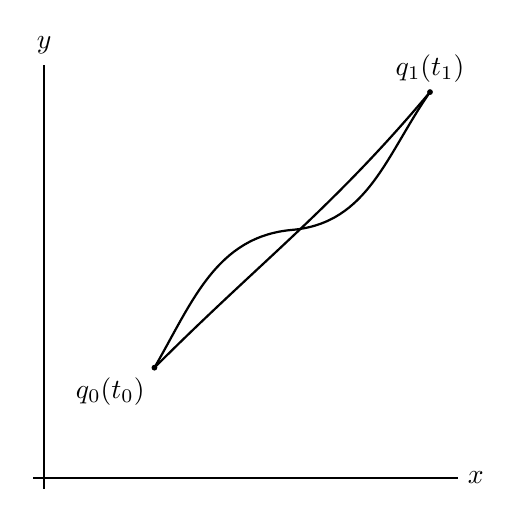
\begin{tikzpicture}[scale=0.7]

    % Draw the axes
    % The axes in the image cross slightly, so we extend them a bit past the origin
    \draw[thick] (-0.2, 0) -- (7.5, 0) node[right] {$x$} ;
    \draw[thick] (0, -0.2) -- (0, 7.5) node[above] {$y$};

    % Define the coordinates for the two points
    \coordinate (P1) at (2, 2);
    \coordinate (P2) at (7, 7);

    % Draw the bottom curve
    % It sags slightly below a straight line between the two points
    \draw[thick] (P1) to[out=45, in=230] (P2);

    % Draw the top curve
    % It has an S-shape, so we use an intermediate point to create the inflection
    \draw[thick] (P1) to[out=60, in=185] (4.5, 4.5) to[out=5, in=235] (P2);

    % Draw the points and their labels
    \fill (P1) circle (1.5pt) node[below left] {\(q_0(t_0)\)};
    \fill (P2) circle (1.5pt) node[above] {\(q_1(t_1)\)};

\end{tikzpicture}
    \caption{Caption}
    \label{fig:placeholder}
\end{figure}

此时，由于时间是整个系统演化的独立自由参数，但作用量又不依赖于该参数演化，意味着作用量可以写为某个量对自由独立参数的积分，即
\begin{equation}
     \action [q]=  \int_{t_1} ^{t_2} \lag(q,\dot{q},t) ~\bd t 
\end{equation}
这个量$\lag$即为\textbf{Lagrangian}。其中Lagrangian可以表示为时间$t$、广义坐标$q$以及广义速度$\dot{q}$的函数。广义速度即为广义坐标$q$对独立自由参数$t$的微分，即
\begin{equation}
    \dot{q} = \frac{\bd q(t)}{\bd t}
\end{equation}
我们可以看到，Lagrangian只包含了路径以及其一阶导数项，却并不显含更高阶的导数项。实际上，系统的运动状态可以由坐标和速度完全确定，因此Lagrangian中并不需要包含更高阶的导数项也足够描述完整的运动信息。

当我们有了最小作用量原理以及这个作用量的形式之后，我们便会去问：如何才能求解系统的真实路径？我们可以先假定$q(t)$是真实的路径，也就是这个\eqref{eq:1stprinciple}式的解，那么我们可以假定存在一个虚位移$\delta q$（路径变分），则会产生一条新的路径为$q+\delta q$，则对应的Lagrangian与真实Lagrangian之间的差值为$\delta\lag$，即
\begin{equation}
    \delta\lag = \frac{\partial\lag}{\partial q}\delta q + \frac{\partial\lag}{\partial \dot q}\delta \dot q 
\end{equation}
也就是说Lagrangian的差值一方面来自于虚位移产生的路径改变，另一方面来自于路径改变之后产生的广义速度改变。在通常的认知中，人们会认为路径与速度似乎总是相互关联的，而不存在两者之间相互独立的情形，但是在这里的泛函变分过程中，我们是在对路径函数的具体形式进行求解，在这时候，这个路径函数的函数值（即广义坐标取值）以及其导数值（广义速度取值）都是未知变量，因此可以对它们进行独立的变分。
而由于时间是一个独立于路径选择的自由参数，因此并不存在$\delta\lag/\delta t$。对于广义速度的变分，我们认为变分和微分都是线性操作，可以交换顺序，因此可以写为
\begin{equation}
    \delta\dot q = \frac{\bd }{\bd t}\delta q
\end{equation}
那么我们可以带入到\eqref{eq:1stprinciple}式中，得
\begin{equation}
    \delta\action[q] = \int_{t_1}^{t_2}\left[ \frac{\partial\lag}{\partial q}\delta q + \frac{\partial\lag}{\partial \dot q}\frac{\bd }{\bd t}\delta q  \right] ~\bd t=0
\end{equation}
对于第二项，我们可以进行分部积分，得到
\begin{equation}
    \delta\action[q] = \frac{\partial\lag}{\partial \dot q}\delta q\Bigg|_{t_1}^{t_2}- \int_{t_1}^{t_2}\left[ \frac{\bd }{\bd t} \left(\frac{\partial\lag}{\partial \dot{q}} \right) -\frac{\partial\lag}{\partial q}  \right] \delta q~\bd t=0
\end{equation}
其中第一项是边界项，通常而言，我们会在初始状态与终止状态已经确定的情况下，去求解未知的运动过程，那么在$t_1$和$t_2$时刻下的函数都为固定常数。然而固定常数项在求解极值时并不产生贡献，因此我们只需要确保第二项积分为0，即可满足作用量取极值的条件，则我们可得
\begin{equation}
    \frac{\bd}{\bd t} \left(\frac{\partial\lag}{\partial \dot{q}} \right)-\frac{\partial\lag}{\partial q}  = 0
\end{equation}
这意味着，只要路径能满足上述方程，即为作用量取极值的路径，也就是真实的路径，那么这便是我们要求解的运动方程，也即称为Euler-Lagrange方程。

值得注意的是，在得到运动方程的过程中，我们会舍去作用量中的常数边界项，而从另一角度来说，实际上作用量并不唯一，当作用量添加任意常数项时，并不改变运动方程。因此我们需要明确的是，运动方程才是实际具有物理意义的，与真实物理路径一一对应，而作用量并不是一个可观测的物理量。同样的逻辑，实际上Lagrangian也不是可观测的物理量，而Lagrangian可以添加任意全微分项，仍能保持运动方程不变
\begin{equation}
    \lag(q,\dot q,t) \rightarrow \lag(q,\dot q,t) + \frac{\bd }{\bd t}\Lambda(q,\dot q,t)
\end{equation}
所以，作用量和Lagrangian都是用来帮助我们去寻找求解运动方程的辅助量。而只有当运动方程保持不变时，我们才能认为真实的物理没有发生变化，即使作用量或者Lagrangain发生变换。但是反过来说，如果作用量或者Lagrangian没有发生变化，那么自然运动方程也不会改变。
\section{约束系统}
\label{sec:constraint}
对于一个存在$N$个质点的力学系统，在经典无约束的情形下每个质点的路径都需要用3个坐标来描述，那么系统的广义坐标的个数就是$3N$个，即为系统的\textbf{自由度}$s$。作用量可以表示为
\begin{equation}
    \action = \action[q_1,\cdots,q_s]
\end{equation}
但是如果存在一定的约束，一部分质点并不是在三维空间中任意运动的，而是在平面上，或者是线上运动的，那么此时系统总的自由度$s$就会小于$3N$个。

意味着有$s$个自由度时，同样也有$s$个广义速度。那么对于多自由度体系来说，可以表示为
\begin{equation}
    \action [q_1,\cdots,q_s] = \int_{t_1} ^{t_2} \lag(q_1,\cdots,q_s,\dot{q}_1,\cdots,\dot q_s;t) ~\bd t 
\end{equation}

\section{Euler-Lagrange方程}
\label{sec:eom}
在此之前，我们只讨论了广义的Lagrangian，而没有讨论到Lagrangian的具体形式。我们可以参照此前对Maupertuis原理[ref]以及虚功原理[ref]的讨论，我们可以给出
\begin{equation}
    \lag = T+W
\end{equation}


第一类Lagrange方程\cite{Lagrange1788a}
\begin{equation}
    \frac{\delta T}{\delta q_\alpha} + \sum_\mu \lambda_\mu \frac{\partial f_\mu}{\partial q_\alpha}=-Q_\alpha
\end{equation}


如果当我们研究的是一个保守系统
系统的做功都为保守力，也即只有势能做功，那么Lagrangian可以表示为
\begin{equation}
    \lag = T - V
\end{equation}

第二类Lagrange方程
\begin{equation}
    \frac{\bd}{\bd t} \left(\frac{\partial\lag}{\partial \dot{q}} \right)-\frac{\partial\lag}{\partial q}  = 0\label{eq:eqomot}
\end{equation}

我们可以看到，实际上Euler-Lagrangian方程给出的运动方程与Newtonian运动方程一致，很多人会因此疑惑，为什么我们需要通过这一套泛函分析的流程绕一大圈才得到我们已知的定律？其实这种泛函分析的流程不仅仅是让我们得到运动方程，更重要的是给出了一套获得运动方程的框架。通常来说，我们只需要带入边界条件通过求解偏微分方程，就能解出运动方程的解，而泛函分析则是用来求解“运动方程的形式”，只有知道运动方程的具体形式之后，才能继续通过解微分方程来获取具体的物理量。在Newtonian力学中，通常运动方程的形式相对简单，能够之间观察出来，但是在经典物理之外，具体的物理问题往往要比Newtonian运动定律中的质点运动学要复杂的多，运动方程所满足的条件形式也复杂多变，而泛函分析恰恰提供了一种能够找到方程形式的数学工具。这一套强大的框架不仅仅是囊括了我们生活中的物理，更是包含了描述微观的粒子以及宏观的宇宙的规律进来，为物理学的研究提供了最基础的语言。

\section{相对性原理}
\label{sec:Galilean}
当我们去构建力学系统时，我们必须要回答的一个问题就是“力学规律在哪个参考系中成立”。一般来说，力学规律在不同的参考系中会有不同的形式，如果没有选择一个较为合适的参考系，那么运动方程的描述将会较为繁琐。

在一般的参考系中，时空缺乏足够的对称性：空间呈现出非均匀性和各向异性，时间也非均匀流逝。这意味着，物体在空间中的不同位置、不同朝向以及不同时刻，其力学表现是不等价的。这种复杂的时空背景会导致一个直观的物理困境：即使是一个不受任何外力作用的自由物体，其运动状态也会显得毫无规律（例如在某一时刻速度为零，下一时刻却发生无端漂移），从而极大地增加了力学描述的复杂度。

然而，物理世界中确实存在一类具有高度对称性的参考系：相对于这类参考系，空间是均匀且各向同性的，时间也是均匀的。我们将这种具有完美时空对称性的参考系定义为\textbf{惯性参考系}。在惯性系的框架下，物理定律能够退去冗余的“坐标伪装”，展现出最简化的数学形式；同时，自由物体在此类参考系中严格遵循其惯性本质——若其在某一时刻处于静止，则将在未来所有时刻保持静止。这正是我们需要引入惯性参考系的核心动因。

Galilean变换
\begin{equation}
    \vec{r} \rightarrow \vec{r}'= \vec{r} +\vec{v}t,~~~~t \rightarrow t' = t
\end{equation}

\begin{figure}[h]
    \begin{tikzpicture}[
    >=Stealth, % Use Stealth arrowheads
    line width=0.8pt,
    font=\large
]

    % === Coordinate System S (Origin O) ===
    \coordinate (O) at (0,0);
    \draw[->] (O) -- (-2.14,-2.14) node[below left] {\(x\)};
    \draw[->] (O) -- (3,0) node[below right] {\(y\)};
    \draw[->] (O) -- (0,3) node[left] {\(z\)};
    \node[left] at (O) {\(O\)};
    \node at (1.2, 2.5) {\(S\)};

    % === Coordinate System S' (Origin O') ===
    \coordinate (Oprime) at (5,1);
    \draw[->] (Oprime) -- ++(-2.14,-2.14) node[below left] {\(x'\)};
    \draw[->] (Oprime) -- ++(3.,0) node[right] {\(y'\)};
    \draw[->] (Oprime) -- ++(0,3) node[above] {\(z'\)};
    \node[below] at (Oprime) {\(O'\)};
    \node at (8, 3) {\(S'\)};

    % === Point P (Tip of the vector) ===
    \coordinate (P) at (3.3, 3);

    % === Vectors ===
    % Vector r (from O to P)
    \draw[->, thick] (O) -- (P) node[midway, above left] {\(\vec{r}\)};
    
    % Vector R (from O to O')
    \draw[->, thick] (O) -- (Oprime) node[midway, above] {\(\vec{R}\)};
    
    % Vector r' (from O' to P)
    \draw[->, thick] (Oprime) -- (P) node[midway, above right] {\(\vec{r}\,'\)};


   

\end{tikzpicture}
\end{figure}



\section{运动积分与N\"other定理}
\label{sec:noether_theo}
对于一个系统的运动方程，我们通常需要带入进边界条件才能够求解出对应的真实运动路径。而在求解微分方程的过程中，这些边界条件最终会贡献到解的一项系数上去。如果边界条件是固定值，即不依赖时间时，那么这些系数也就会是一些积分常数。
而我们也可以发现，实际上存在某些物理量，它只依赖于初始的状态的函数，而在整个运动过程中保存不变，那么这些物理量恰好会成为最终运动方程解的一部分积分常数，也是首次积分，即称之为运动积分。

当我们考虑系统的Lagrangian不显含时间时，意味着$ \frac{\partial\lag}{\partial t }=0$，那么Lagrangian没有特定时间的取向，Lagrangian在时间分布上是均匀的，这也就是\textbf{时间平移对称性}。那么我们可以考察Lagrangian的时间全微分
\begin{equation}
    \frac{\bd \lag }{\bd t} = \sum_\alpha^s \frac{\partial\lag}{\partial q_\alpha}\dot q_\alpha + \sum_\alpha^s \frac{\partial\lag}{\partial \dot q_\alpha}\ddot q_\alpha
\end{equation}
其中$\frac{\partial\lag}{\partial q_\alpha}$可以利用运动方程\eqref{eq:eqomot}式进行替换，可得
\begin{equation}
    \frac{\bd \lag }{\bd t} = \sum_\alpha^s \frac{\bd }{\bd t}\left(\frac{\partial\lag}{\partial \dot q_\alpha} \right) \dot q_\alpha + \sum_\alpha^s \frac{\partial\lag}{\partial \dot q_\alpha}\ddot q_\alpha = \sum_\alpha^s \frac{\bd }{\bd t}\left(\frac{\partial\lag}{\partial \dot q_\alpha}\dot q_\alpha \right)
\end{equation}
那么我们可以得到
\begin{equation}
     \sum_\alpha^s \frac{\bd }{\bd t}\left(\frac{\partial\lag}{\partial \dot q_\alpha}\dot q_\alpha -\lag\right) = 0
\end{equation}
此时该全微分为0，意味着该物理量在时间演化中是守恒的，而这个守恒量在实际物理过程中我们定义为“\textbf{能量}”，
\begin{equation}
    E =  \sum_\alpha^s \frac{\partial\lag}{\partial \dot q_\alpha}\dot q_\alpha -\lag\label{eq:energy}
\end{equation}
而对于\eqref{eq:energy}该等式，实际上已经将作为二阶微分方程的运动方程转化为一个一阶的微分方程，带入Lagrangian的经典形式，我们可以解得
\begin{equation}
    E = \frac{1}{2}m \dot q^2 + V(q)
\end{equation}
那么此时我们可以直接进行积分去求解该微分方程
\begin{equation}
    t = \int_{q_1}^{q_2} \sqrt{\frac{m}{2[E-V(q)]}}~\bd q
\end{equation}
最终可以反解出路径函数$q(t)$。


\begin{theorem}[N\"other erster Satz]
    Gestattet die erste Variation eines Integrals eine endliche kontinuierliche Gruppe von \(q\) wesentlichen Parametern, so werden \(q\) lineare Verbindungen der Lagrangeschen Ableitungen des Integrals zu Divergenzen.\\ Insbesondere kennt man also im eindimensionalen Falle, wo die Divergenzen zu totalen Differentialquotienten werden, \(q\) erste Integrale der durch Nullsetzen der ersten Variation gegebenen Differentialgleichungen.
\end{theorem}

\begin{theorem}[N\"other zweiter Satz]
Gestattet die erste Variation eine unendliche kontinuierliche Gruppe mit \(q\) willkürlichen Funktionen, so besteht zwischen den Lagrangeschen Ableitungen und ihren Differentialquotienten \(q\) lineare Beziehungen,\\ so daß \(q\) Gleichungen eine Folge der übrigen werden. 
\end{theorem}

\section{质点运动学}

对于一个在三维空间不受约束的质点而言，其Lagrangian可以描述为
\begin{equation}
    \lag = \frac{1}{2}m\dot{\vec{r}}^2 - V(\vec{r})
\end{equation}
这时其速度矢量可以在具体坐标系中展开，例如我们最常用的直角坐标系，也称为Cartesian坐标系，在该坐标系下，质点粒子的位移可以用$(x,~y,~z)$三个相互正交的坐标来描述。那么，质点粒子无穷小位移矢量模方可以表示为
\begin{equation}
    |\bd \vec{r}|^2 = \bd x^2 + \bd y^2 + \bd z^2 = \begin{pmatrix}
        \bd x,~\bd y,~\bd z
    \end{pmatrix}\begin{pmatrix}
        1& & \\
        & 1& \\ 
        & & 1
    \end{pmatrix}\begin{pmatrix}
         \bd x\\\bd y\\\bd z
    \end{pmatrix}
\end{equation}
那么自然对于速度，我们可以利用上式获得位移矢量在此坐标系下的时间导数，带入到Lagrangian即为
\begin{equation}
    \lag = \frac{1}{2} m  (\dot x^2 +\dot y^2 + \dot z^2) - V(x,y,z)
\end{equation}
在此参考系中，我们可以对各个方向去求解运动方程，得
\begin{equation}
    % \begin{split}
        m\ddot x =- \frac{\partial V}{\partial x},~~~~%\\
          m\ddot y =- \frac{\partial V}{\partial y},~~~~%\\
            m\ddot z =- \frac{\partial V}{\partial z}
    % \end{split}
\end{equation}
此时，我们考虑质点粒子的广义动量
\begin{equation}
    p_x = \frac{\partial\lag}{\partial \dot x} = m\dot x，~~~~ p_y = \frac{\partial\lag}{\partial \dot y} = m\dot y，~~~~ p_z = \frac{\partial\lag}{\partial \dot z} = m\dot z
\end{equation}

当我们考虑质点在$x-y$平面上存在一定得圆周运动时，可以用柱坐标系来描述质点的运动，也就是在$x,~y$平面用半径$r$与方位角$\phi$来描述，即$\vec{r} = (r,~\phi,~z)$。
那么柱坐标系下的无穷小的位移矢量模方可以表示为
\begin{equation}
    |\bd\vec{r}|^2 = \bd r ^2 + r^2 \bd \phi^2 + \bd z ^2
\end{equation}
利用该微分得到速度项，带入到Lagrangian中，我们可得
\begin{equation}
    \lag = \frac{1}{2} m  (\dot r^2 +r^2\dot \phi^2 + \dot z^2) - V(r,\phi,z)
\end{equation}
那么可得运动方程
\begin{align}
    % \begin{split}
        &m(\ddot r - r\dot\phi^2) = -\frac{\partial V}{\partial r}\\
        &mr(r\ddot \phi + 2\dot r \dot\phi)  = -\frac{\partial V}{\partial \phi}\\
        &m\ddot z = -\frac{\partial V}{\partial z}
    % \end{split}
\end{align}
而对于广义动量，我们有
\begin{equation}
    p_r  = m\dot r,~~~~~~~~
    p_\phi = mr^2\dot\phi ,~~~~~~~~
    p_z = m\dot z
\end{equation}
其中对于方位角相对应的广义动量$p_\phi$，其量纲与普通的动量不同，比其他动量多一个长度的量纲。而$p_\phi$正是质点的角动量$L=mr^2\dot\phi$。


球坐标系
\begin{equation}
    \lag = \frac{1}{2} m  (\dot r^2 +r^2\dot \theta^2 + r^2\sin^2\theta \dot \phi^2)
\end{equation}

\begin{figure}[h]
    \centering
 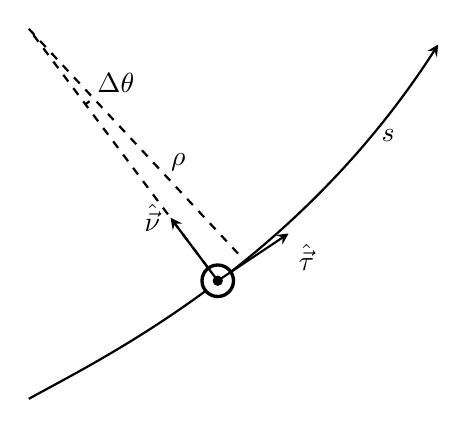
\begin{tikzpicture}[>=stealth, scale=1.0]

    % % Background ruled lines
    % \foreach \y in {-2,-1,0,1,2,3} {
    %     \draw[gray!30, very thin] (-4,\y) -- (4,\y);
    % }

    % Path S
    \draw[thick, ->] (-2.4,-1.5) .. controls (-1.5,-1.0) and (1.0,0.2) .. (2.8, 3.0) node[pos=0.85, right] {\(s\)};

    % Dashed lines
    % Extension of velocity vector
    \draw[dashed, thick] (0,0) -- (-2.4, 3.2); 
    % Line towards center of curvature P
    \draw[dashed, thick] (-2.4, 3.2) -- (0.3,0.3) ; 

    % Angle Delta Theta
    % Angle of v extension: atan2(3.2, -2.4) = 126.87 degrees
    % Angle of P line: atan2(2.7, 1.6) = 59.35 degrees
    \draw[thick] (-2.4,3.2) ++(126.87:-1.2) arc (126.87:130:-1.2) node[pos=0.4, above right] {\(\Delta \theta\)};

    % Particle (circle with inner dot)
    \draw[very thick, fill=white] (0,0) circle (0.2);
    \filldraw[thick] (0,0) circle (0.05); 

    % Velocity vector v
    \draw[->, thick] (0,0) -- (-0.6, 0.8) node[left] {\(\hat{\vec{\nu}}\)};

    % Change in velocity vector Delta v
    \draw[->, thick] (0,0) -- (0.9, 0.6) node[below right] {\(\hat{\vec{\tau}}\)};

    % % Angle beta
    % % Tangent backward angle: atan2(-1.6, 1.2) = -53.13 degrees
    % \draw[thick] (0,0) ++(0:0.6) arc (0:-53.13:0.6);
    \node at (-0.5,1.5) {\(\rho\)};

\end{tikzpicture}
    \caption{Caption}
    \label{fig:placeholder}
\end{figure}

\chapter{Hamiltonian力学}

\section{Hamiltonian正则方程}
\label{sec:cannoical_eqs}
考虑对Lagrangian做Legendre变换，将广义速度$\dot q$的依赖变换为广义动量$p$的依赖
\begin{equation}
    \ham(q,p,t) = p\dot q - \lag(q,\dot q, t),~~~~p = \frac{\partial\lag}{\partial\dot q}
\end{equation}
变换后的量称之为Hamiltonian。那么对Hamiltonian做变分可得
\begin{equation}\begin{split}
     \bd \ham = \bd(p\dot q) - \bd \lag=p\,\bd\dot q + \dot q\, \bd p-\frac{\partial\lag}{\partial q}\bd q -\frac{\partial\lag}{\partial\dot q}\bd \dot q - \frac{\partial\lag}{\partial t}\bd t\\
     % &=\dot q\delta p - \frac{\partial\lag}{\partial q}\delta q\\
     % &
\end{split}
\end{equation}
带入Euler-Lagrange方程，即
\begin{equation}
    \frac{\partial\lag}{\partial q} = \frac{\bd}{\bd t}\frac{\partial\lag}{\partial\dot q},~~p = \frac{\partial\lag}{\partial\dot q}
\end{equation}
可得
\begin{equation}
    \begin{split}
       \bd\ham & = \dot q 
       \,\bd p - \dot p \,\bd q-\frac{\partial\lag}{\partial t}\bd t\\&=\frac{\partial\ham}{\partial p}\bd p +  \frac{\partial\ham}{\partial q}\bd q + \frac{\partial\ham}{\partial t}\bd t
    \end{split}
\end{equation}
那么我们可整理得
\begin{equation}
    \frac{\partial\ham}{\partial p} = \dot{q},\qquad\frac{\partial \ham}{\partial q} = -\dot{p},\qquad \frac{\partial\ham}{\partial t} = -\frac{\partial\lag}{\partial t}
\end{equation}
其中如果Lagrangian不显含时间，那么Hamiltonian也不显含时间。对于不显含时间的情形，我们可得到方程组
\begin{equation}
    \begin{cases}
        \frac{\partial\ham}{\partial p} = \dot{q}\\
        \frac{\partial \ham}{\partial q} = -\dot{p}
    \end{cases}
\end{equation}
这便是Hamiltonian正则方程组。该方程组同样描述着运动方程，但是与Euler-Lagrange方程不同的是，它将原来的二阶微分方程转化为两个一阶微分方程组，这种形式在面对较为复杂的系统上方便人们进行迭代求解。

值得注意的是，现在Hamiltonian的变量变成了广义坐标以及广义动量，而由广义坐标与广义动量张成的空间称之为\textit{{相空间}}，在相空间中的每一个点上，动量和坐标都是确定的，因此每一个点上都一一对应着系统的一个运动状态。随着时间演化，系统在相空间中也产生出一条一条的轨迹，然而有趣的是，这些描述系统运动的轨迹是不会相交的，这意味着对于某一时刻的系统处于某一运动状态时，下一时刻的运动状态是确定的。如果相空间轨迹出现相交，那么相交点的时刻下系统则会出现两种“未来”。这意味着相空间并不像普通的线性空间一样，而是会存在一定的特殊结构，称之为\textit{辛几何（Sympletic Geometry）}。

% \section{相空间与辛几何}
\section{运动方程降维法}
Routhian 
\begin{equation}
    \mathcal{R} = \sum_{j=1}^l \dot q_j p_j - \lag(q_{l+1},q_{l+2}\cdots q_s, \cdot q_1, \cdots\cdot q_s, t)
\end{equation}

\section{Poisson括号}
\label{sec:poisson_brak}
对于任意力学量$f(q,p,t)$，其对于时间的全微分可以写为
\begin{equation}
    \frac{\bd f}{\bd t} = \frac{\partial f}{\partial t} + \sum_\alpha^s\left( \frac{\partial f}{\partial q_\alpha}\dot q_\alpha + \frac{\partial f}{\partial p_\alpha}\dot p_\alpha \right)
\end{equation}
带入Hamiltonian正则方程，可得
\begin{equation}
    \frac{\bd f}{\bd t}= \frac{\partial f}{\partial t}+\sum_\alpha^s\left( \frac{\partial f}{\partial q_\alpha}\frac{\partial\ham}{\partial p_\alpha} - \frac{\partial f}{\partial p_\alpha}\frac{\partial\ham}{\partial q_\alpha} \right)
\end{equation}
其中我们将后两项的计算可以定义Poisson括号，即任意两力学量$g,~f$的Possion括号即为
\begin{equation}
    \{g,f\} = \sum_\alpha^s\left( \frac{\partial f}{\partial q_\alpha}\frac{\partial g}{\partial p_\alpha} - \frac{\partial f}{\partial p_\alpha}\frac{\partial g}{\partial q_\alpha} \right)
\end{equation}
那么力学量$f$的全微分可以写为
\begin{equation}
    \frac{\bd f}{\bd t} = \frac{\partial f}{\partial t} + \{\ham,f\}\label{eq:poissondef}
\end{equation}
对于任意不显含时间的力学量$f$，即$\frac{\partial f}{\partial t}=0$，当我们有
\begin{equation}
    \{ f,\ham\} = 0
\end{equation}
则$\dot f=0$，力学量$f$是一个守恒量，即运动积分。

如果我们考虑广义动量和广义坐标的Poisson括号，将带入到广义动量和广义坐标到\eqref{eq:poissondef}式中，我们可以发现，Hamiltonina正则方程组还可以写为如下形式
\begin{equation}
    \begin{cases}
        \dot q_\alpha = \{ q_\alpha,\ham\}\\
        \dot p_\alpha = \{p_\alpha, \ham \}
    \end{cases}
\end{equation}
而对于广义动量和广义坐标之间做Poisson括号，我们可得
\begin{equation}
    \{ q_\alpha, q_\beta\}=0,\qquad\{ p_\alpha, p_\beta\}=0,\qquad \{ q_\alpha, p_\beta\} = \delta_{\alpha\beta}
\end{equation}

Poisson可以看成是一种代数运算，具有如下性质
\begin{itemize}
    \item [i.] $\{f,~\mathrm{const.}\}=0$
    \item [ii.] $C\{f,~g\}=\{Cf,~g\} = \{f,~Cg\}$
    \item [iii.] $\{f,~g\}=-\{g,~f\}$
    \item [iv.] $\{f,~g_1+g_2\}=\{f,~g_1\}+\{f,~g_2\}$
    \item [v.] $\{f,~g_1 g_2\} = \{f,~g_1\}g_2 + g_1 \{f,~g_2\}$
    \item [vi.] $\frac{\partial }{\partial t}\{f,~g\} = \{\frac{\partial f}{\partial t},~g\} + \{f,~\frac{\partial g}{\partial t}\}$
\end{itemize}

\section{正则变换}
\label{sec:cannoical_transf}
对于一个在相空间中定义且满足Hamiltonian正则方程$\ham(q_\alpha,p_\alpha,t)$的力学系统，我们可以对相空间坐标进行坐标变换
\begin{equation}
    (q_\alpha,~p_\alpha)\mapsto (Q_\alpha,~P_\alpha),~~~~\ham(q_\alpha,p_\alpha,t)\mapsto \mathcal{K}(Q_\alpha,P_\alpha,t)
\end{equation}
那么新的Hamiltonian依然满足正则方程
\begin{equation}
    \dot Q_\alpha = \frac{\partial \mathcal{K}}{\partial p_\alpha},~~~~\dot P_\alpha = -\frac{\partial\mathcal{K}}{\partial q_\alpha}
\end{equation}
其中新的正则动量以及正则坐标依赖于原坐标与动量
\begin{equation}
    Q = Q(q,p,t),~~~~P=P(q,p,t)
\end{equation}
那么相空间的Jacobian可以表为
\begin{equation}
    M = \frac{\partial(Q,P)}{\partial(q,p)}
\end{equation}
新的正则坐标依然保持相空间的辛结构
\begin{equation}
    J = \begin{pmatrix}
        0&  \mathbbm{1}\\
        -\mathbbm{1}& 0
    \end{pmatrix},~~~~M^T J M = J
\end{equation}
同时，新的正则坐标也满足Poisson括号
\begin{equation}
    \{Q_\alpha,~Q_\beta\} = 0, ~~~~\{P_\alpha,~P_\beta\} = 0, ~~~~\{Q_\alpha,~P_\beta\} = \delta_{\alpha\beta}
\end{equation}

在进行了正则变换后，Hamiltonian的变换可以表示为
\begin{equation}
    \mathcal{K} = \ham + \frac{\partial\mathcal{F}}{\partial t}
\end{equation}
其中$\mathcal{F}$称之为正则变换的生成函数。生成函数有四类，分别为
\begin{itemize}
    \item {第一类生成函数} $\displaystyle \mathcal{F}_1=(q,Q,t),\qquad ~~~~ p_\alpha = \frac{\partial\mathcal{F}_1}{\partial q_\alpha},~~~~P_\alpha = -\frac{\partial\mathcal{F}_1}{\partial Q_\alpha}$
    \item {第二类生成函数} $\displaystyle \mathcal{F}_2=(q,P,t),\qquad ~~~~ p_\alpha = \frac{\partial\mathcal{F}_2}{\partial q_\alpha},~~~~Q_\alpha = \frac{\partial\mathcal{F}_2}{\partial P_\alpha}$
    \item {第三类生成函数} $\displaystyle \mathcal{F}_3=(p,Q,t),\qquad ~~~~ q_\alpha = -\frac{\partial\mathcal{F}_3}{\partial p_\alpha},~~~~P_\alpha =- \frac{\partial\mathcal{F}_3}{\partial Q_\alpha}$
    \item {第四类生成函数} $\displaystyle \mathcal{F}_4=(p,P,t),\qquad ~~~~ q_\alpha = -\frac{\partial\mathcal{F}_4}{\partial p_\alpha},~~~~Q_\alpha = \frac{\partial\mathcal{F}_4}{\partial P_\alpha}$
\end{itemize}

% \section{Louville定理}
\section{Hamilton-Jacobi方程}
\label{sec:Ham_Jacobi}
我们重新回顾到作用量，如果我们将作用量看成是起点固定，但是终点待定的情形，此时作用量可以表示为显含时间的函数
\begin{equation}
    \action(q,t) = \int_{t_0}^{t}\lag(q,\dot q,\tau)\bd \tau
\end{equation}
那么对于作用量的全微分，包含了Lagrangian的微分贡献以及路径变分的贡献，即
\begin{equation}
    \bd \action(t) = \lag(t)\bd t + \int_{t_0}^{t}\delta\lag(q,\dot q,\tau)\bd\tau = \lag(t)\bd t + \int_{t_0}^{t}\left( \frac{\partial\lag}{\partial q}\delta q + \frac{\partial\lag}{\partial \dot q}\delta\dot q \right)\bd\tau 
\end{equation}
此时进行分部积分，那么边界项将会因为末端时间$t$未定而保留$\delta q(t)$项，但是$\delta q(t_0)$因为是固定处态而是0，最后带入运动方程，可得
\begin{equation}
    \bd \action(t) = \lag(t)\bd t+\frac{\partial\lag}{\partial\dot q}\delta q\Bigg|^t_{t_0} = \lag(t)\bd t+p\,\delta q(t)\label{eq:drvhjeq1}
\end{equation}
对于末端时刻$t$的路径的全微分，其包含了路径本身的变分，以及时间微分项的贡献，即
\begin{equation}
    \bd q =\delta q(t) + \dot q \bd t 
\end{equation}
则
\begin{equation}
    \delta q(t) = \bd q-\dot q \bd t 
\end{equation}
带入回\eqref{eq:drvhjeq1}式，即可得
\begin{equation}
    \bd \action(t) = \lag(t)\bd t+p( \bd q-\dot q \bd t ) = (\lag - p\dot q)\bd t + p\bd q  = -\ham \bd t  +p\bd q
\end{equation}
其中利用了Lagrangian可以通过Legendre变换获得Hamiltonian得关系。而作用量得全微分可以表示为
\begin{equation}
    \bd\action = \frac{\partial\action}{\partial q}\bd q + \frac{\partial\action}{\partial t}\bd t
    \end{equation}
    那么我们可以得到对应得关系
    \begin{equation}
        p = \frac{\partial\action}{\partial q},\qquad \ham = - \frac{\partial\action}{\partial t}
    \end{equation}
    由于此时，Hamiltonian是关于广义坐标$q$和广义动量$q$得函数，但是此时广义动量可以从上式中表示，那么带入到Hamiltonian中，我们最终可以得到以下方程
\begin{equation}
    \ham\left(q,~\frac{\partial\action}{\partial q},~t\right) + \frac{\partial \action}{\partial t}=0
\end{equation}
这就是Hamilton-Jacobi方程，是一个关于作用量$\action$函数得一阶微分方程。求解出作用量函数的具体形式，则可以求去求解路径$q$。

当我们考虑Hamiltonian不显含时间的情形，那么作用量则可以写成能量积分的形式
\begin{equation}
    \action (q_1,\cdots q_s,t) = \mathcal{W}(q_1,\cdots q_s)-Et,\qquad \ham = - \frac{\partial\action}{\partial t} = E
\end{equation}
此时则将作用量函数进行了分离变量，$\mathcal{W}$则称为Jacobi作用量。那么Hamilton-Jacobi方程则可化为
\begin{equation}
    \ham\left(q_1,\cdots q_s,~\frac{\partial\mathcal{{W}}}{\partial q_1},\cdots \frac{\partial\mathcal{{W}}}{\partial q_s} \right) = E
\end{equation}
